\documentclass[
size=17pt,
paper=smartboard,
mode=present,
display=slidesnotes,
style=sailor,
nopagebreaks,
blackslide,
fleqn]{powerdot}
 %wj capsules prettybox
 %mode = handout or present

\usepackage{amsmath,graphicx,color,amsfonts}
\usepackage[brazilian]{babel}
\usepackage[utf8]{inputenc}

\pdsetup{
   lf = {EC01045 PDS},
   rf = {Sinais e Sistemas Discretos},palette ={Sea},randomdots={false}
}
% palette = {green}, 

%opening
\title{\Large EC01045 -- Processamento Digital de Sinais\\ \vspace{1cm}Sinais e Sistemas Discretos}
\author{Ronaldo de Freitas Zampolo\\FCT-ITEC-UFPA}
\date{ }

\begin{document}
   
   \maketitle[randomdots={false}]
   \begin{slide}{Agenda}
      \tableofcontents[content=sections]
   \end{slide}

\section[slide=false]{Sinais discretos}
\begin{slide}{Sequências básicas 3}
   \begin{itemize}
     \item Exponencial:
     \onslide*{1-3}{
     \begin{equation}
         x[n]=A\alpha^n
         \label{eq:expo}
     \end{equation}}
     \onslide*{2-3}{
     Em geral, $A$ e $\alpha$ são complexos:
     \begin{align}
         A &=|A|e^{j\phi} \label{eq:A}\\
         \alpha &= |\alpha|e^{j\omega_o}
         \label{eq:Alpha}
     \end{align}}
     \onslide*{3}{
     Substituindo (\ref{eq:A}) e (\ref{eq:Alpha}) em (\ref{eq:expo}),
      \begin{align*}
          x[n] & = |A||\alpha|^n e^{j(\omega_o n+\phi)}\\
               & = |A||\alpha|^n \left [  \text{cos}(\omega_o n+\phi) + j\text{sen}(\omega_o n+\phi)\right ]
      \end{align*}}
      \onslide*{4}{
         $x[n]=0,9^n$\\
         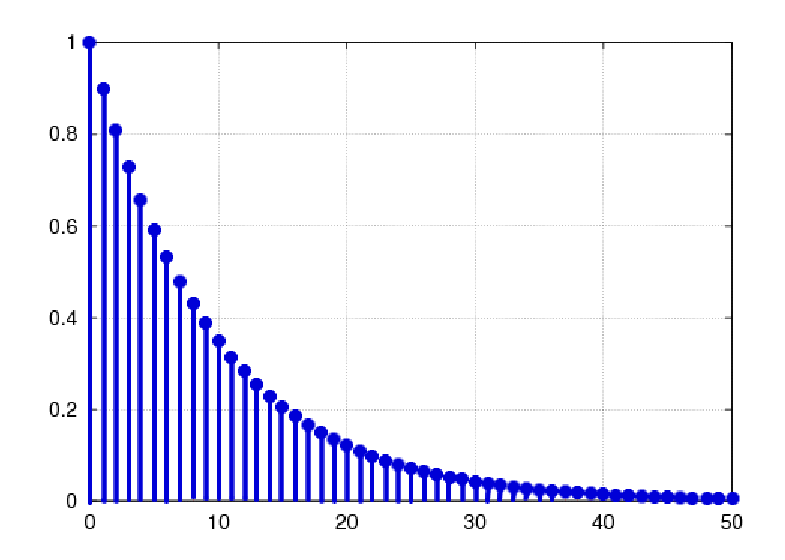
\includegraphics[width=0.7\textwidth]{figs/expo1.eps}}
       \onslide*{5}{
         $x[n]=1,1^n$\\
         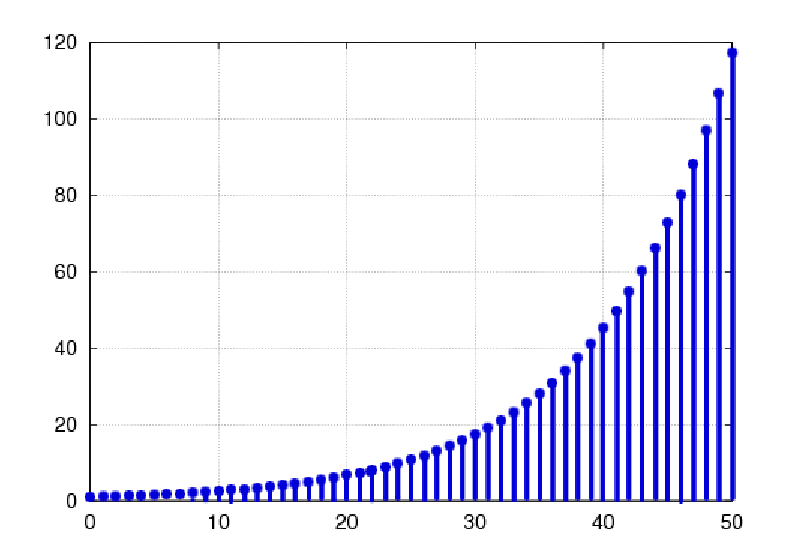
\includegraphics[width=0.7\textwidth]{figs/expo2.eps}}
       \onslide*{6}{
          $x[n]=\cos\left (\frac{\pi}{16}n \right )$\\
          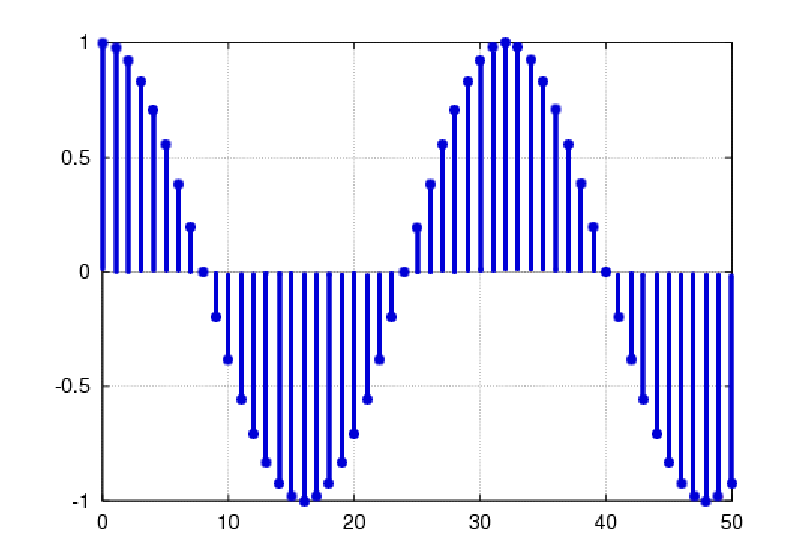
\includegraphics[width=0.7\textwidth]{figs/expo3.eps}}
       \onslide*{7}{
          $x[n]=0,7^n\cos\left (\frac{\pi}{16}n \right )$\\
          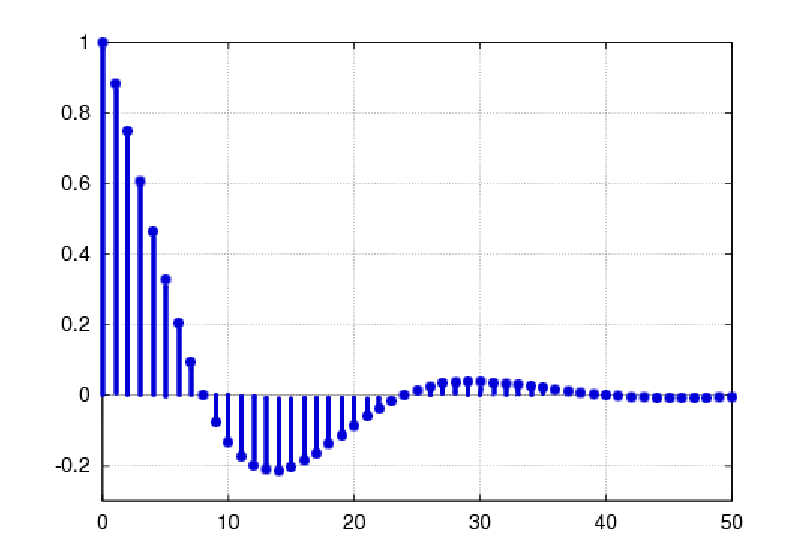
\includegraphics[width=0.7\textwidth]{figs/expo4.eps}}
       \onslide*{8}{
          $x[n]=1,1^n\cos\left (\frac{\pi}{16}n \right )$\\
          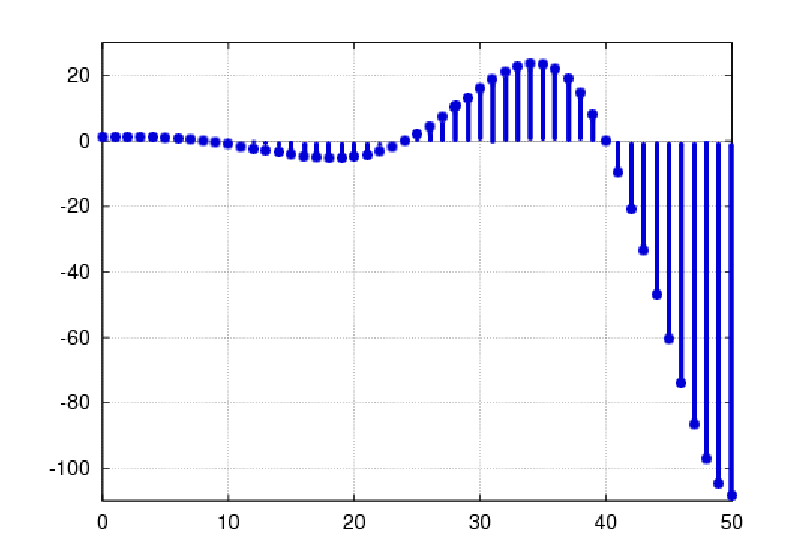
\includegraphics[width=0.7\textwidth]{figs/expo5.eps}}
       \end{itemize}
\end{slide}

 \begin{slide}{Sinais $e^{j\omega n}$: periodicidade em $\omega$ }
    \begin{itemize}
     \item <1-4> Considere um sinal do tipo $e^{j\omega_o n}$, onde $\omega_o$ representa um valor de ``frequência'' específico
     \item <2-4> O que acontece se formos aumentando o valor de $\omega_o$?
     \item <3-4> Chegará um momento em que 
        \begin{equation*}
             \omega_f = \omega_o + 2\pi
        \end{equation*}
        \begin{equation*}
        \begin{split}
           e^{j\omega_f n} & = e^{j(\omega_o + 2\pi)n} \\
                           &=e^{j\omega_o n}
         \end{split}
        \end{equation*}
        \begin{itemize}
           \item <4>\textcolor{red}{Não há distinção entre as ``frequências'' $\omega_o$ e $\omega_o+2\pi$}
     \end{itemize}
   \end{itemize}
 \end{slide}
 
 
\begin{slide}{Sinais $e^{j\omega n}$: periodicidade em $\omega$ }
   \begin{itemize}
    \item %Periodicidade em $\omega$:
    \onslide*{1}{$\omega_1 = 0$; $\omega_2 = 2\pi$ 
    \begin{center}
     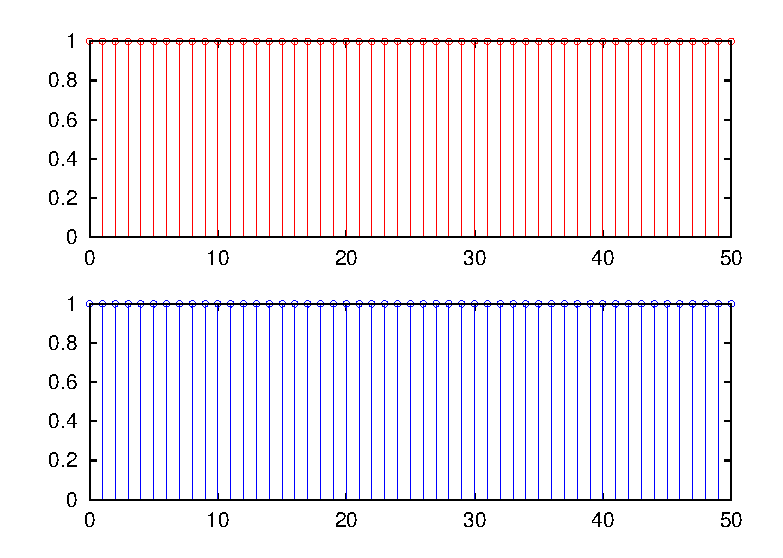
\includegraphics[width=0.7\textwidth]{figs/perfreq01.eps}
    \end{center}}
    \onslide*{2}{$\omega_1 = \frac{\pi}{4}$; $\omega_2 = \frac{9\pi}{4}$ 
    \begin{center}
     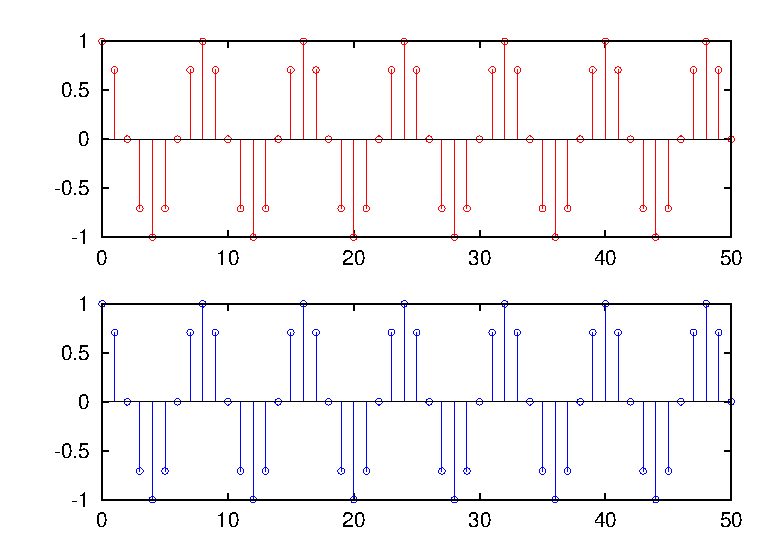
\includegraphics[width=0.7\textwidth]{figs/perfreq02.eps}
    \end{center}}
    \onslide*{3}{$\omega_1 = \frac{\pi}{3}$; $\omega_2 = \frac{7\pi}{3}$ 
    \begin{center}
     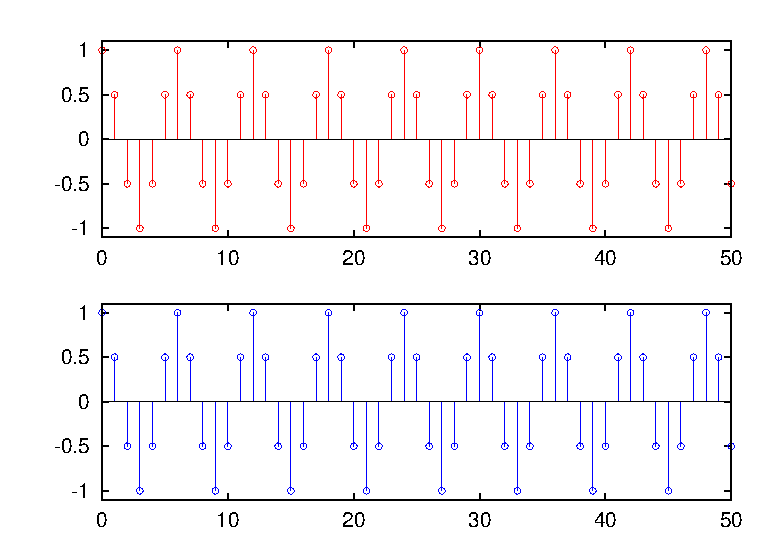
\includegraphics[width=0.7\textwidth]{figs/perfreq03.eps}
    \end{center}}
   \onslide*{4}{$\omega_1 = \frac{\pi}{1,1}$; $\omega_2 = \frac{3,2\pi}{1,1}$ 
    \begin{center}
     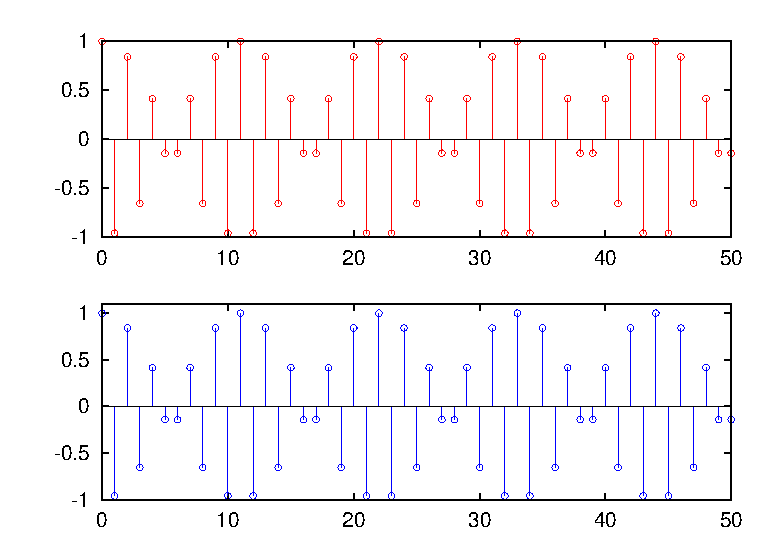
\includegraphics[width=0.7\textwidth]{figs/perfreq04.eps}
    \end{center}}
   \onslide*{5}{O deslocamento de $2\pi$ faz com que se volte ao ``mesmo ponto''
    \begin{center}
     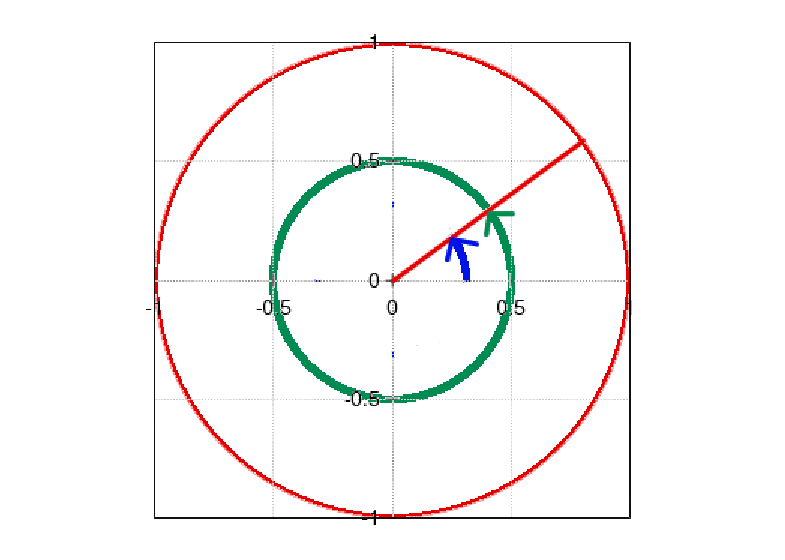
\includegraphics[width=0.8\textwidth]{figs/perfreq_circ.eps}
    \end{center}}
   \end{itemize}
\end{slide}
 
\begin{slide}{Sinais $e^{j\omega n}$: periodicidade em $n$ }
   \begin{itemize}
    \item <1-3> Considerando um sinal do tipo $e^{j\omega_o n}$, onde $\omega_o$ representa um valor de ``frequência'' específico
     \item <2-3> Que condições tal sinal deve possuir para ser periódico em $n$?
     \item <3-3> Se $e^{j\omega_o n}$ é periódico em $n$ com período $N$,
        \begin{align*}
           e^{j\omega_o n} &= e^{j\omega_o (n+N)}\\
                           &= e^{j\omega_o n} e^{j\omega_o N}\\
        %\end{align*}
        %\onslide*{4}{
        %\begin{align*}
             \omega_o N &= k2\pi, \quad N, k \in \mathbb{Z}\\
               \omega_o &= \frac{k2\pi}{N} \Rightarrow \frac{\omega_o}{2\pi} = \frac{k}{N}\quad k=0,1,\ldots, N-1
         \end{align*}%}
     %Há, assim, um número \textcolor{red}{finito} de sinais periódicos $e^{j\omega_o}$ distintos: $k=0,1,\ldots, N-1$
%     \end{itemize}
%  \end{itemize}
\end{itemize}
\end{slide} 

\begin{note}{O número de sinais exponenciais periódicos}
   Há, assim, um número \textcolor{red}{finito} de sinais periódicos $e^{j\omega_o}$ distintos: $k=0,1,\ldots, N-1$
\end{note}


\begin{slide}{Sinais $e^{j\omega n}$: periodicidade em $n$ }
   \begin{itemize}
    \item Exemplos:
    \onslide*{1}{
     $\omega = \frac{\pi}{7}$
    \begin{center}
     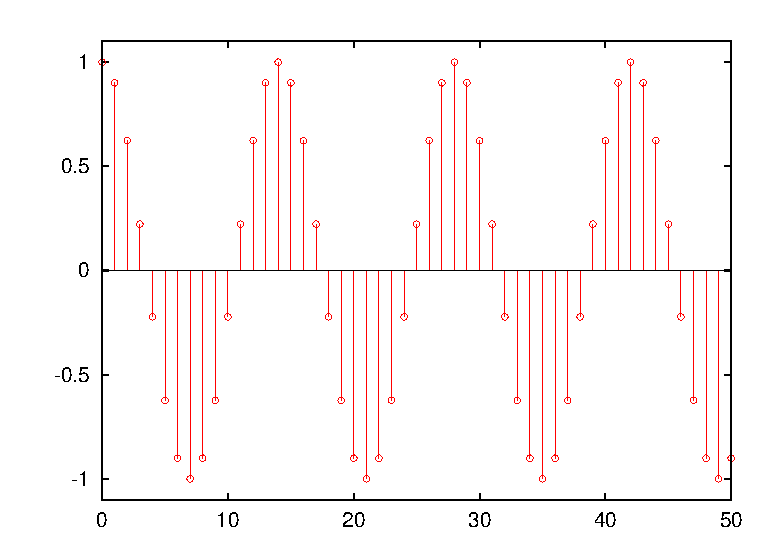
\includegraphics[width=0.7\textwidth]{figs/perfn01.eps}
    \end{center}}
    \onslide*{2}{
     $\omega = 0,45$ 
    \begin{center}
     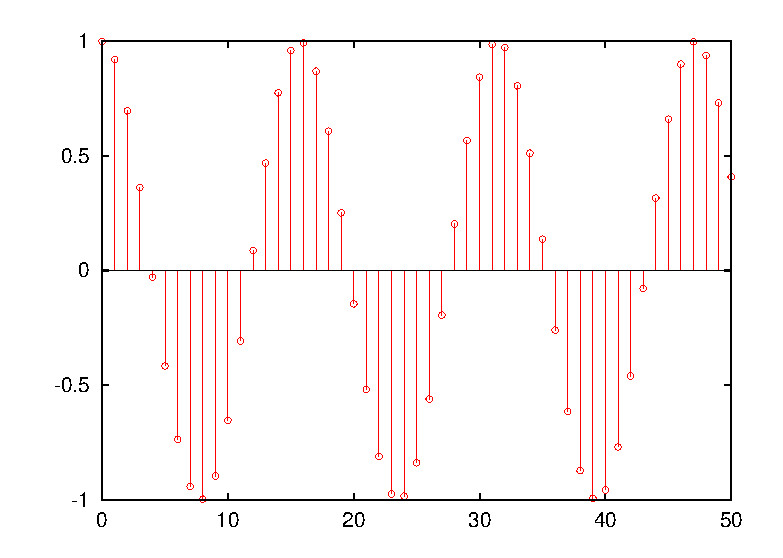
\includegraphics[width=0.7\textwidth]{figs/perfn02.eps}
    \end{center}}
   \end{itemize}
\end{slide}

\section[slide=false]{Sistemas discretos}
\begin{slide}{Definições}
   \begin{itemize}
   \item <1->Mapeamento entre entrada e saída de um sistema
    \setlength{\unitlength}{1cm}
    \begin{center}
    \begin{picture}(4,1)
      \thicklines
      \put( 0, 0.5 ) {\vector(1,0){1}}
      \put( 1, 0 ) {\framebox( 2, 1){T\{$\bullet$\}}}
      \put( 3, 0.5 ) {\vector(1,0){1}}
      
      \put(0.2,0){$x$}
      \put(3.2,0){$y$}
      
    \end{picture}
    \end{center}

    \item <2->Sistemas sem memória: saída atual $y[n]$ depende somente da entrada atual $x[n]$
    \item <3->Sistemas invariantes: 
    \begin{align*}
        y_1[n] &=\text{T}\{x_1[n]\}\\
        y_2[n] &=\text{T} \{x_2[n]\} \\
               &=\text{T} \{x_1[n-n_o]\}= y_1[n-n_o]\\
      \end{align*}
  \end{itemize}
\end{slide}

\begin{slide}{Invariância: exemplos}
   \begin{itemize}
   \item Sistemas invariantes -- Exemplo:
   \onslide*{1} {
   \begin{center}
     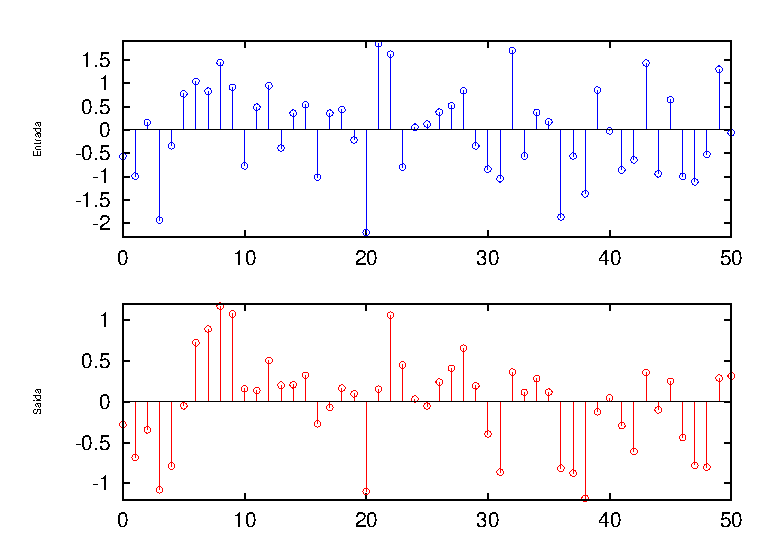
\includegraphics[width=0.7\textwidth]{figs/invariante01.eps}
    \end{center}}
   \onslide*{2} {
   \begin{center}
     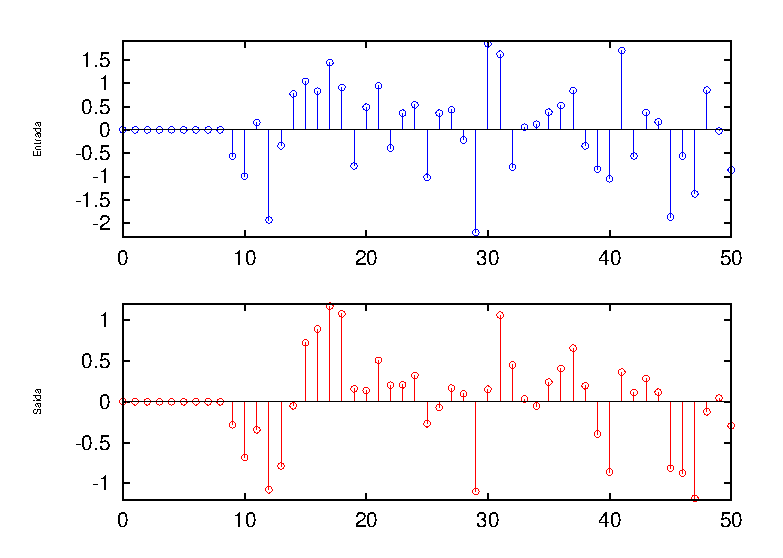
\includegraphics[width=0.7\textwidth]{figs/invariante02.eps}
    \end{center}}
   \end{itemize}
\end{slide} 

\begin{slide}{Causalidade e estabilidade}
   \begin{itemize}
    \item <1->Causalidade: a saída $y[n_o]$ depende das entradas $x[n]$, onde $n \leq n_o$
    \item <2>Estabilidade: BIBO (\textit{bounded-input bounded-output})\\
    \begin{align*}
       |x[n]| \leq B_x < \infty, \quad \forall n\\
       |y[n]| \leq B_y < \infty, \quad \forall n
    \end{align*}

  \end{itemize}
\end{slide}


\begin{slide}{Sistemas lineares}
   \begin{itemize}
        
%     \item Sistemas lineares:
%     \begin{itemize}
       \item <1->Princípio da homogeneidade:
       \begin{equation*}
        \text{T}\{\alpha x[n]\} = \alpha \text{T}\{ x[n]\}
       \end{equation*}
       \item <2->Princípio da aditividade:
       \begin{equation*}
           \text{T}\{x_1[n]+x_2[n]\} = \text{T}\{x_1[n]\} + \text{T}\{x_2[n]\}
       \end{equation*}
       \item <3>\textcolor{red}{Princípio da superposição:}
       \begin{equation*}
     \text{T}\{\alpha x_1[n] + \beta x_2[n] \}= \alpha \text{T}\{x_1[n]\} + \beta \text{T}\{x_2[n]\}
    \end{equation*}
    \end{itemize} 
%   \end{itemize}
\end{slide}

% %\begin{slide}{Sistemas discretos}
% %   \begin{itemize}
% %    \item Tarefa 01: Classifique quanto à linearidade, causalidade e variância
% %    \scriptsize{
% %    \begin{align}
% %       y[n]&=x[n-n_d], \quad -\infty<n<\infty\\
% %       y[n]&=\frac{1}{M_1+M_2+1}\sum_{k=-M_1}^{M_2}x[n-k]\\
% %       y[n]&=(x[n])^2\\
% %       y[n]&=\sum_{k=-\infty}^{n}x[k]\\
% %       y[n]&=x[Mn]\\
% %       y[n]&=x[n+1]-x[n]\\
% %       y[n]&=x[n]-x[n-1]
% %    \end{align}}
% %
% %   \end{itemize}
% %\end{slide}

\section[slide=false]{Sistemas lineares e invariantes} 
\begin{slide}{Mapeamento entre entrada e saída 1}
   \begin{itemize}
    \item <1->Resposta $y[n]$ de um sistema LI ao sinal $x[n]$
    \begin{align*}
        y[n]&=\text{T}\left \{ x[n] \right \}\\
            &=\text{T}\left \{ \sum_{k=-\infty}^{\infty}x[k]\delta [n-k] \right \}.
    \end{align*}
     \item <2-> Usando o \emph{princípio da superposição},
     \begin{align*}
        y[n]&=\sum_{k=-\infty}^{\infty}x[k]\text{T}\left \{ \delta [n-k] \right \}\\
            &=\sum_{k=-\infty}^{\infty}x[k]h_k[n].
     \end{align*}
   \end{itemize}
\end{slide}


\begin{slide}{Mapeamento entre entrada e saída 2}
   \begin{itemize}
    \item <1->Considerando o sistema invariante,
    \begin{align*}
        y[n]&=\sum_{k=-\infty}^{\infty}x[k]h_k[n]\\
            &=\sum_{k=-\infty}^{\infty}x[k]h[n-k].
     \end{align*}
     \onslide*{2}{Soma (somatório) de convolução:
     \begin{equation*}
         \boxed{y[n]=\sum_{k=-\infty}^{\infty}x[k]h[n-k]}
     \end{equation*}}
   \end{itemize}
\end{slide}

% \begin{note}{Interpretações da convolução}
% Há três maneiras de considerar a convolução:
% \begin{itemize}
%    \item Interpretação gráfica tradicional (atenção aos intervalos do somatório)
%    \item Interpretação gráfica considerando a resposta do sistema aos impulsos correspondentes às amostras do sinal de entrada
%  \item Formação de tabela (boa estratégia para sinais pequenos e finitos)
% \end{itemize}
% \end{note}
% 
% \begin{note}{Exercícios de convolução}
% \begin{enumerate}
% \item Exercício: calcule $y[n]= h[n]*x[n]$, onde 
%    
%    \begin{enumerate}
%       \item $h[n]=u[n]-u[n-3] \qquad \text{e} \qquad x[n]=\left ( \frac{3}{4} \right )^nu[n]$
%       \item $h[n]=u[n]-u[n-3] \qquad \text{e} \qquad x[n]=u[n]-u[n-2]$
%       \item $h[n]=\begin{cases} \frac{1}{2}, & n=-1\\
%                                 1,           & n=0\\
%                                 \frac{1}{2}, & n=1\\
%                                 0,           & \text{outro caso}
%                    \end{cases} $\\
%              $x[n]=\begin{cases} a[n], & n\text{ par}\\
%                                   0,   & n\text{ ímpar}
%                    \end{cases}$
%    \end{enumerate}
% \end{enumerate}
% \end{note}
\end{document}
